\documentclass[../../memoria.tex]{subfiles}

\begin{document}

\paragraph{}
La primera de estas pruebas ha consistido en utilizar el comando time \cite{timelinuxcom} para poder medir el tiempo que tarda el \textit{MVP} en desplegarse y comenzar a funcionar. Se ha ejecutado mediante el comando time el script launch\_tfg.sh tres veces, así como sobre el script destroy\_tfg.sh otras tres veces. De esta forma se puede comprobar cuánto tiempo tarda, de media, en desplegarse y cuánto en destruirse. Los resultados de estas pruebas han sido los siguientes:

\begin{figure}[H]
    \centering
    \begin{minipage}{.5\textwidth}
        \centering
        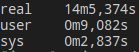
\includegraphics[width=0.6\columnwidth]{pruebaApply1.png}
        \caption{launch\_tfg.sh. Prueba 1}
        \label{fig:pruebaApply1}
    \end{minipage}%
    \begin{minipage}{.5\textwidth}
        \centering
        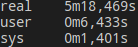
\includegraphics[width=0.6\columnwidth]{pruebaDestroy1.png}
        \caption{destroy\_tfg.sh. Prueba 1}
        \label{fig:pruebaDestroy1}
    \end{minipage}
\end{figure}

\begin{figure}[H]
    \centering
    \begin{minipage}{.5\textwidth}
        \centering
        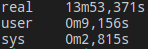
\includegraphics[width=0.6\columnwidth]{pruebaApply2.png}
        \caption{launch\_tfg.sh. Prueba 2}
        \label{fig:pruebaApply2}
    \end{minipage}%
    \begin{minipage}{.5\textwidth}
        \centering
        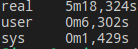
\includegraphics[width=0.6\columnwidth]{pruebaDestroy2.png}
        \caption{destroy\_tfg.sh. Prueba 2}
        \label{fig:pruebaDestroy2}
    \end{minipage}
\end{figure}

\begin{figure}[H]
    \centering
    \begin{minipage}{.5\textwidth}
        \centering
        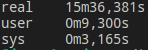
\includegraphics[width=0.6\columnwidth]{pruebaApply3.png}
        \caption{launch\_tfg.sh. Prueba 3}
        \label{fig:pruebaApply3}
    \end{minipage}%
    \begin{minipage}{.5\textwidth}
        \centering
        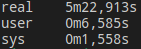
\includegraphics[width=0.6\columnwidth]{pruebaDestroy3.png}
        \caption{destroy\_tfg.sh. Prueba 3}
        \label{fig:pruebaDestroy3}
    \end{minipage}
\end{figure}

\paragraph{}
Como se puede observar en las imágenes, el sistema tarda de media algo menos de quince minutos en desplegarse completamente. Este despliegue es de infraestructura y del simulador. A partir de ese momento, el simulador ya comienza a enviar datos al IoT Core.

\paragraph{}
También puede observarse que tarda de media algo más de cinco minutos en destruirse por completo.

\paragraph{}
Por lo tanto, tras esta prueba se pueden sacar las siguientes conclusiones:

\begin{enumerate}
    \item Desplegar un sistema en la nube (AWS en este caso) utilizando infraestructura como código es un proceso muy ágil. Se ha conseguido desplegar un sistema complejo, con una base de datos como es Elasticsearch en menos de 15 minutos.
    \item Destruir el sistema creado es incluso más rápido. Además, utilizando \textit{IaC}, no se corre el riesgo de olvidar algún recurso sin destruir que consuma presupuesto de manera indeseada.
    \item En este caso, con AWS y Terraform, los tiempos tanto de despliegue como de destrucción varían muy poco, por lo que se pueden asegurar rangos de tiempos para ambos procesos eficazmente.
\end{enumerate}
\end{document}
